%
% File acl2021.tex
%
%% Based on the style files for EMNLP 2020, which were
%% Based on the style files for ACL 2020, which were
%% Based on the style files for ACL 2018, NAACL 2018/19, which were
%% Based on the style files for ACL-2015, with some improvements
%%  taken from the NAACL-2016 style
%% Based on the style files for ACL-2014, which were, in turn,
%% based on ACL-2013, ACL-2012, ACL-2011, ACL-2010, ACL-IJCNLP-2009,
%% EACL-2009, IJCNLP-2008...
%% Based on the style files for EACL 2006 by 
%%e.agirre@ehu.es or Sergi.Balari@uab.es
%% and that of ACL 08 by Joakim Nivre and Noah Smith

\documentclass[11pt,a4paper]{article}
\usepackage[hyperref]{acl2021}
\usepackage{times}
\usepackage{latexsym}
\usepackage{graphicx}
\graphicspath{ {./} }
\renewcommand{\UrlFont}{\ttfamily\small}

% This is not strictly necessary, and may be commented out,
% but it will improve the layout of the manuscript,
% and will typically save some space.
\usepackage{microtype}

\aclfinalcopy
%\def\aclpaperid{***} %  Enter the acl Paper ID here

%\setlength\titlebox{5cm}
% You can expand the titlebox if you need extra space
% to show all the authors. Please do not make the titlebox
% smaller than 5cm (the original size); we will check this
% in the camera-ready version and ask you to change it back.

% Content lightly modified from original work by Jesse Dodge and Noah Smith


\newcommand\BibTeX{B\textsc{ib}\TeX}

\title{Project Report, CS598 DL4H in Spring 2023}

\author{Manu Vinod Shesha \\
  \texttt{manuv3@illinois.edu}
  \\[2em]
  Group ID: 96\\
  Paper ID: 187\\
  Presentation link: \url{TODO} \\
  Code link: \url{https://github.com/manuv3/cs598-dl-project}} 

\begin{document}
\maketitle

% All sections are mandatory.
% Keep in mind that your page limit is 8, excluding references.
% For specific grading rubrics, please see the project instruction.

\section{Introduction}

This work reproduces the idea and results in the original paper: \textit{Automated ICD-9 Coding via A Deep Learning Approach}\cite{8320340}.

The original paper aims to automate the extraction of ICD-9 (Ninth Revision of International Classification of Diseases) codes from patient discharge summary, through application of general text processing technique called Document-to-Vector (D2V) in combination of Convolution Neural Network (CNN).

The extraction of ICD-9 codes from free-text Discharge summary is needed to do billing, as well as raising insurance claims with the provider. Today, the procedure to extract medical codes from patient discharge summary is largely a manual effort, undertaken by hospital’s medical record department personnel. This has two problems:
\begin{itemize}
    \item The process is very slow and inefficient, causing delay in the patient discharge process.
    \item The process requires specialized knowledge making it costly, and sometimes error prone.
\end{itemize}

The authors describe a novel approach to this problem through usage of DL techniques. They treat it as a task of multi-label classification (of ICD-9 codes). Specifically, the authors combine two approaches to produce vector embedding of documents, which are further used in multi-label classification:
\begin{itemize}
    \item CNN (Convolution Neural Network) to discover, and extract \textbf{local features} in text. We can Intuitively, the local context of the text, like phrases describing a medical concept, should be important in deriving related ICD codes.
    \item D2V (Document to Vector) \cite{le2014distributed} embedding technique to capture the \textbf{global features} of the document. D2V extends upon Word2Vec, and (unlike CNN) takes order of words into account. It should be noted that D2V unsupervised learning approach.
\end{itemize}



\section{Scope of reproducibility}

The paper claims that proposed DL model combining Doc2Vec (D2V) and CNN, generates better embedding for documents, which in-turn perform better in multi-label classification task of identifying ICD-9 codes, when compared to traditional ML-based models.  

More specifically, it claims:

\begin{itemize}
	\item Higher Micro-average F1-score in multi-label ICD-9 classification task for the proposed model when compared to baseline models: Flat-SVM and Hierarchical-SVM.
\newline

\begin{small}
\begin{tabular}{ cccc }
  \hline
  	Model & Precision & Recall & F1-score \\
  \hline
  	flat-SVM & 0.635 & 0.158 & 0.253 \\ 
  \hline
  	hierarchical-SVM & 0.415 & 0.280 & 0.335 \\ 
  \hline
  	D2V+CNN & 0.486 & 0.351 & \textbf{.408} \\ 
  \hline
\end{tabular}

\textit{All values are Micro-averaged.}
\end{small}

	\item Each of the components: CNN and D2V provide important contribution to the overall accuracy of the model (, with CNN being more important). The model accuracy degrades significantly when either of these components are removed.
\newline

\begin{small}
\begin{tabular}{ cccc }
  \hline
  	Model & Precision & Recall & F1-score \\
  \hline
  	Only CNN & 0.440 & 0.366 & 0.399 \\ 
  \hline
  	Only D2V & 0.375 & 0.261 & 0.308 \\ 
  \hline
  	D2V+CNN & 0.486 & 0.351 & .408 \\ 
  \hline
\end{tabular}

\textit{All values are Micro-averaged.}
\end{small}	
\end{itemize}
 
\subsection{Addressed claims from the original paper}


\begin{itemize}
    \item Higher Micro-average F1-score in multi-label ICD-9 classification task for the proposed model when compared to baseline models: Flat-SVM and Hierarchical-SVM.
    \item The model accuracy degrades significantly when either of the components: D2V or CNN are removed.
    \item In addition, we also build a different variation of the model which uses CNN with attention (instead of CNN with D2V), as part of additional work to verify if the performance can be improved.
\end{itemize}

\section{Methodology}

\subsection{Model descriptions}
The model is a DL network with two "logical" components: Encoder and Classifier.

The Encoder generates fixed-length embedding for a given discharge summary document.This component consists of two "logical" sub-components: D2V and CNN.

The "D2V" sub-component first trains (as pre-processing step) Doc2Vec model to learn input document vectors of length \texttt{128}, in an unsupervised way. It then fine-tunes these vectors in a supervised way using a fully connected layer of \texttt{64} neurons, followed by a non-linear activation like ReLU (Rectified Linear Unit), and finally, a dropout layer which regularizes the output of fully-connected layer by stochastically dropping different dimensions of the output vector.

The "CNN" sub-component uses Word2Vec as pre-processing step to build word vectors (of size \texttt{100}) for the whole vocabulary of the collective corpus of documents. For each document, all the vectors corresponding to the contained words, are "stacked" as a matrix, to represent the given document. Batches of these document matrices are used as input to the CNN sub-component. This sub-component actually comprises of 3 single-layer multi-channel CNN models, similar to reference implementation in \cite{kim2014convolutional}. Three CNN models correspond to 3 kernel sizes of \texttt{3 (x 100), 4 (x 100), and 5 (x 100)}, with \texttt{64} output channels each. 2D CNN layer in each model is followed by a MaxPool layer to perform temporal pooling. The outputs of each of these CNN models are concatenated to generate the output vector per document of size \texttt{192 (3 models * 64 channels each)}.
    
The ouput vectors from the two sub-components (D2V and CNN) are concatenated to produce the final vector for each document in the batch. Ths final vector size is \texttt{256 (64 from DNN + 192 from CNN)}.

The Classifier performs multi-label classification of ICD-9 codes. This component consists of a fully connected layer with sigmoid activation. This layer generates the final output of size \texttt{6984 (total number of ICD-9 codes)}. Each dimension (representing an ICD-9 code) is assigned a probability by sigmoid activation.


Architecture is summarized in diagram \ref{arch_diag}.

\begin{figure*}
  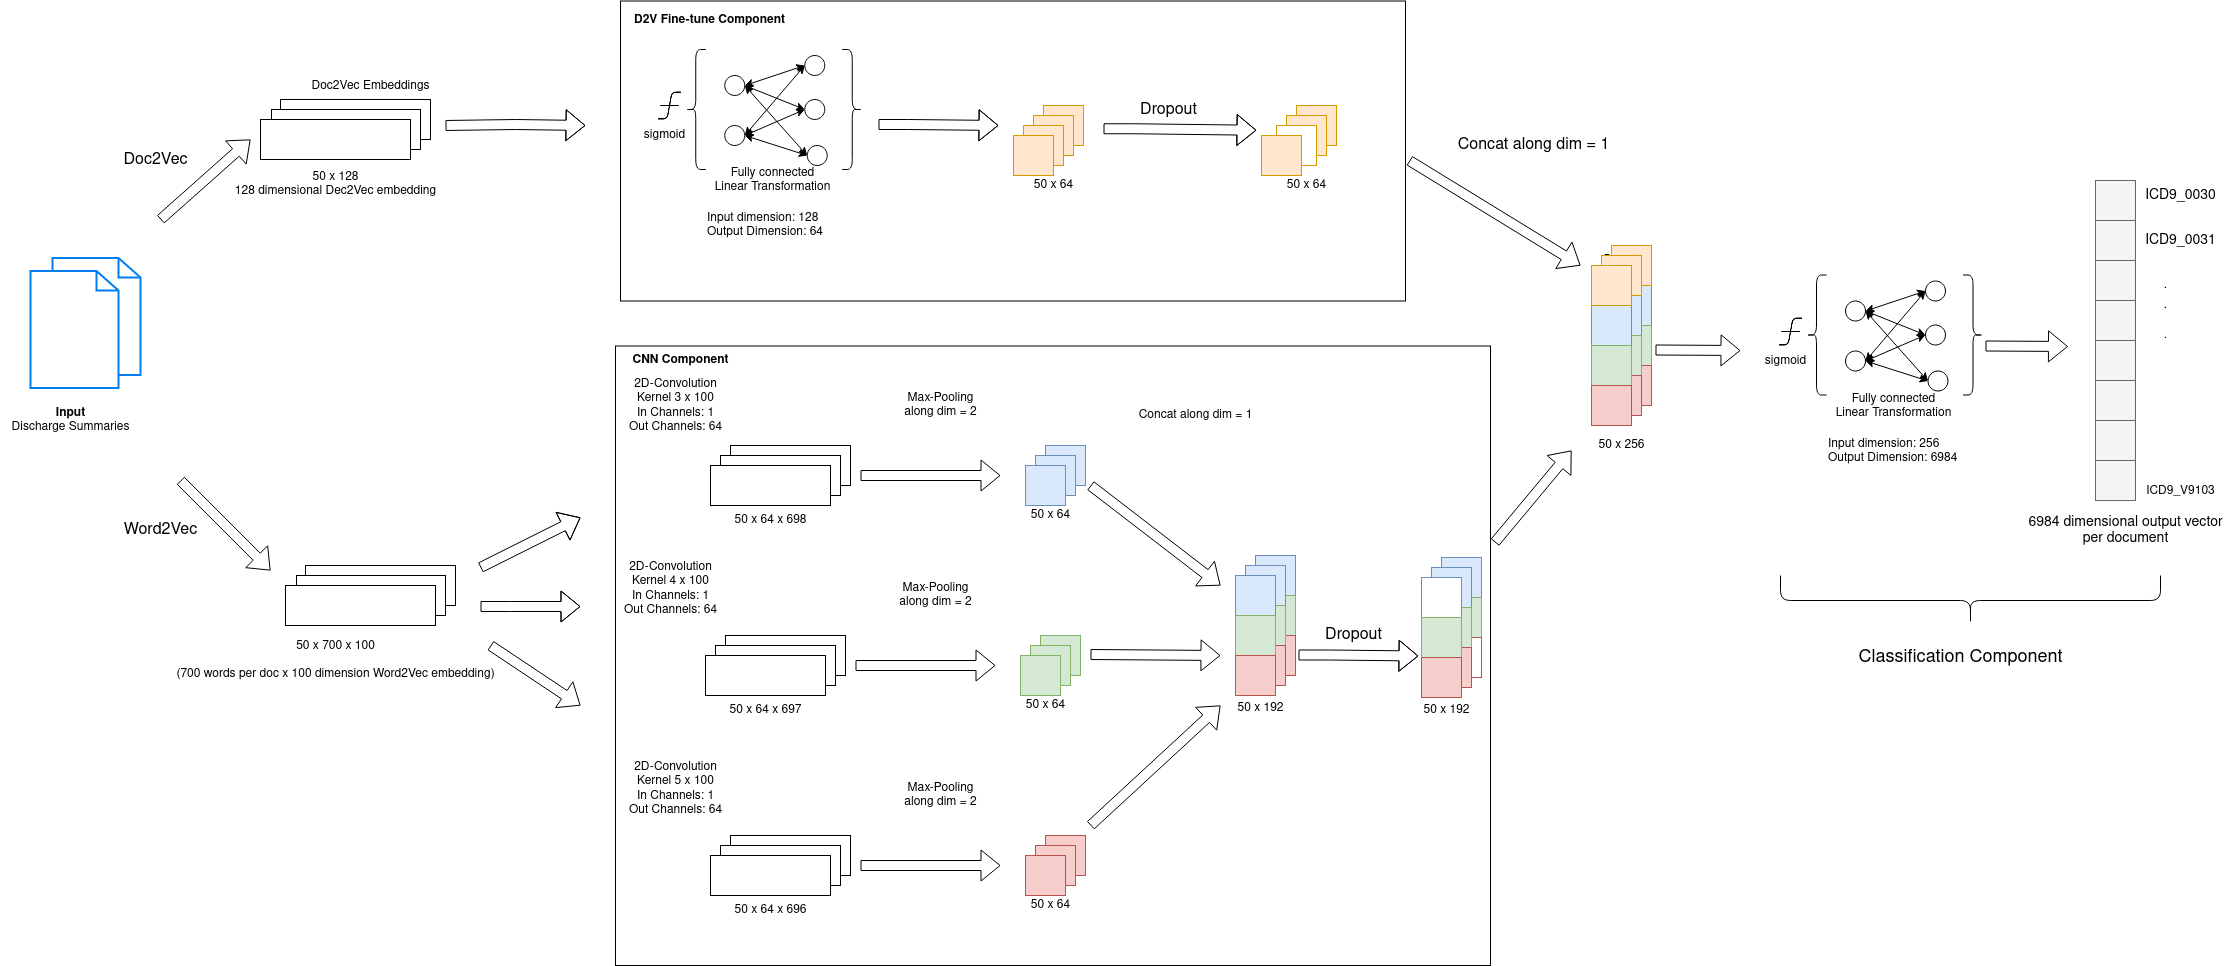
\includegraphics[width=\textwidth,height=4cm]{../src/architecture}
  \caption{D2V + CNN Model Architecture}
  \label{arch_diag}
\end{figure*}
\begin{figure*}
  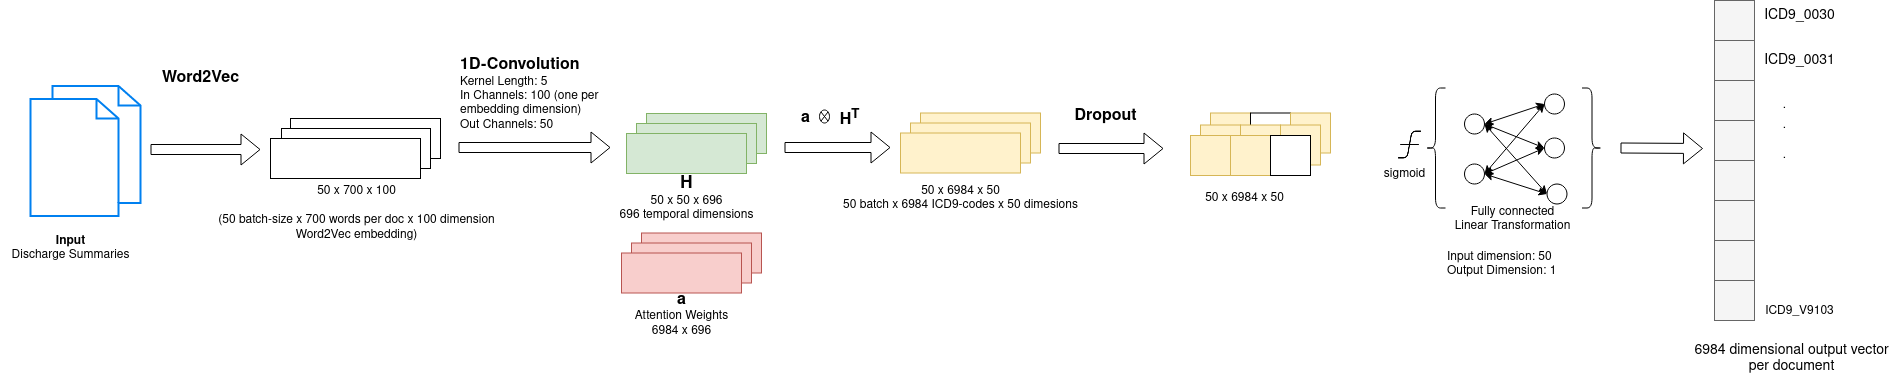
\includegraphics[width=\textwidth,height=4cm]{../src/architecture2}
  \caption{CNN + Attention Model Architecture}
  \label{arch2_diag}
\end{figure*}

The objective is to do end-to-end training of this model. Doc2Vec and Word2Vec models are trained unsupervised, in the pre-processing step. During the supervised learning phase, the above described components are trained for multi-label classification task using back-propagation. The gaol is to achieve similar or close enough performance in terms of micro-averaged F1-score, as achieved in original paper.

The model is medium complexity model in terms of the number of parameters to train.
\newline

\begin{small}
\begin{tabular}{ ll }
  \hline
  	CNN layer (3x100, 4x100, 5x100 sized \\ 2D-kernels with 64 out-channels each) & 76992 \\
  \hline
  	D2V Fine-tune layer \\ (128 input dimension, 64 neurons) & 8256 \\
  \hline
  	Fully-connected classification layer \\ (256 input dimension, 6984 neurons) & 1794888 \\
  \hline
\end{tabular}
\end{small}
\newline

An additional model (not part of the original paper) was created to study the impact of attention over plain CNN. The idea is inspired from CAML\citep{mullenbach-etal-2018-explainable} architecture which leverages attention weights (along with other techniques) to derive ICD-9 codes from MIMIC-III discharge summary reports. The archiecture of this model consists of a single layer multi-channel 1D CNN, an attention mechanism, and finally, the classification component consisting of a fully connected layer with a Sigmoid classifier. Refer to diagram \ref{arch2_diag}. The objective of this experiment was not to build a finely tuned model, but to check if the performance (in terms of micro f1-score) can be improved using attention mechanism.

The table below details the number of parameters in this additional model.
\newline

\begin{small}
\begin{tabular}{ ll }
  \hline
  	CNN layer (3-sized 1D-kernel with 100 \\ in-channels and 50 out-channels) & 25050 \\
  \hline
  	Attention matrix (6984 output states x 696 \\ temporal hidden states) & 349200 \\
  \hline
  	Fully-connected classification layer \\(50 input dimension, 1 output dimension) & 51 \\
  \hline
\end{tabular}
\end{small}


\subsection{Data descriptions}

The model is trained and tested on MIMIC-III \href{https://physionet.org/content/mimiciii/1.4/}{MIMIC-III} (Medical Information Mart for Intensive Care) database. The data is publicaly available, upon credentiating user identity on Physionet, and completing the mandatory training: Data or Specimens Only Research.

Specifically, following datasets in MIMIC-III were used:

\begin{itemize}
    \item DIAGNOSES\_ICD.csv: Each row in this file maps HADM\_ID (Hospitalization ID) of a patient with a unique ICD9\_CODE. We transform ICD9\_CODE to one-hot encoding and group them per per HADM\_ID to generate multi-hot encoding.
\newline

\begin{small}
\begin{tabular}{ ll }
  \hline
  	Total \# codes & 6984 \\
  \hline
  	Avg. \# codes per patient & 11 \\
  \hline
  	Max \# of codes per patient & 39 \\
  \hline
  	Min \# of codes per patient & 1 \\
  \hline
\end{tabular}
\end{small}

	\item NOTEEVENTS.csv: Each row maps HADM\_ID (Hospitalization ID) with a TEXT (free text Discharge summary) field.
\newline

\begin{small}
\begin{tabular}{ ll }
  \hline
    Total \# discharge summary & 52691 \\
  \hline
    Avg. \# words per discharge summary & 1524 \\ 
  \hline
    Max \# of words per discharge summary & 7980 \\
  \hline
  	Min \# of words per discharge summary & 9 \\
  \hline
\end{tabular}
\end{small}
\end{itemize}


\subsection{Hyperparameters}

For the reproducability, following hyperparamters were tuned:
\begin{itemize}
	\item Probabilities for dropout layers in D2V and CNN components: The original paper found the optimum value of dropout probability to be \texttt{0.70}. But in this reproducibility work, the best performance was achieved at \texttt{0.20} dropout probability. 
	\item Threshold value for binary classification: The value between 0 and 1, represents the threshold to assign class 0 or 1 for a given ICD-9 code, in the final classification layer. The original paper found the optimum threshold value as \texttt{0.20}. The same was found to be optimum in this reproducibility work. Lower threshold value was resulting in higher recall but lower accuracy. Similalry higher threshold resulted in higher accuracy but lower recall. At 0.20 threshold, accuracy and recall achieved harmonic balance to result in higher f1-score.
\end{itemize}

Many potential hyperparameters like number of units in fully connected layers (in D2V fine-tuning, and in classification component), convolution kernel sizes, Doc2Vec/Word2Vec embedding dimensions, and max number of tokens per document, were used as described in original paper.

Many "potential hyperparameters like type of activation function (ReLU), learning rate for backward propagation (0.001), etc. were chosen based on "conventional" wisdom and kept constant throughout, due to time constraint, and resource limits.

\subsection{Implementation}

The implemenation has been entirely done by the team. To the best of knowledge of the team, no implementation code by authors of original paper is available publicly.

The implementation uses Jupyter notebooks.

The notebook \href{https://github.com/manuv3/cs598-dl-project/blob/main/src/data\_preprocessing.ipynb}{data\_preprocessing.ipynb} imports the MIMIC-III datasets (\texttt{DIAGNOSES\_ICD.csv} and \texttt{NOTEEVENTS.csv}), applies necessary preprocessing and saves the final datasets.
    \begin{itemize}
    		\item Filtering unnecessary columns from datasets. From \texttt{DIAGNOSES\_ICD.csv}, only \texttt{HADM\_ID, ICD9\_CODE} columns are needed. From \texttt{NOTEEVENTS.csv}, only \texttt{HADM\_ID, TEXT} columns are needed.
    		\item Grouping \texttt{ICD9\_CODE} per hospital visit, and representing them as multi-hot vector.
    		\item Pickling the transformed Pandas Dataframes and saving on disk.
    \end{itemize}

The notebook \href{https://github.com/manuv3/cs598-dl-project/blob/main/src/w2v\_d2v.ipynb}{w2v\_d2v.ipynb} generates and saves following:
	\begin{itemize}
		\item \href{https://radimrehurek.com/gensim/models/word2vec.html}{Gensim Word2Vec} model based vectors for all the tokens in the vocabulary of our corpus.
		\item \href{https://radimrehurek.com/gensim/models/doc2vec.html}{Gensim Doc2Vec} model based vectors for all the documents in our corpus.
	\end{itemize}

\textit{(The above two notebooks are not needed to run the main notebook dl\_model.ipnyb, as all the pre-processed data generated by these two notebooks have been made saved and made available to dl\_model.ipnyb)}
	
The notebook \href{https://github.com/manuv3/cs598-dl-project/blob/main/src/dl\_model.ipynb}{dl\_model.ipynb} trains and validates the DL models (as described in the model section). Following models have been included in this notebook:
		\begin{itemize}
			\item DL full model (D2V + CNN)
			\item D2V-only DL model (ablation)
			\item CNN-only DL model (ablation)
			\item CNN with attention DL model (additional work)
		\end{itemize}

Link to source code: \url{https://github.com/manuv3/cs598-dl-project/tree/main/src}


\subsection{Computational requirements}

Two coumptational environments were used in this work:
\begin{itemize}
	\item Personal Machine: 
	\begin{itemize}
		\item CPU: \texttt{Intel® Core™ i7-10750H × 12 processor with 16.0 GiB Memory}
		\item GPU: \texttt{NVIDIA GeForce GTX 1650 with 4.0 GiB Memory}
	\end{itemize}
	\item Google Collab Free with "standard" GPU support
\end{itemize}


The computational requirements for different steps are described below:
\begin{itemize}
	\item MIMIC-III datasets import and preprocessing: All the steps were performed on personal machine on CPU.
\newline

\begin{small}
\begin{tabular}{ ll }
	\hline
   		Memory used & 10 GiB \\
  	\hline
    		Time taken & 3-4 minutes \\
    \hline
    		Disk space needed for \\ input datasets & 3.75 GB \\
    	\hline
    		Disk space needed for \\ output DataFrames & 876 MB \\		 
  	\hline
\end{tabular}
\end{small}
\newline

	\item Word2Vec and Doc2Vec model training and vectors generation: All the steps were performed on personal machine. Gensim implementaion of Word2Vec and Doc2Vec support streamed source. So, there is no need to load the whole corpus in memory. However, there is no GPU support in Gensim yet.
\newline

\begin{small}
\begin{tabular}{ ll }
	\hline
   		Word2Vec embeddings \\ generation time & 37 minutes \\
  	\hline
    		Doc2Vec embeddings \\ generation time & 51 minutes \\ 
  	\hline
  		Memory used & 1.5 GB \\
  	\hline
  		Disk space needed for \\ output embeddings & 70.1 MB \\
  	\hline
\end{tabular}
\end{small}
\newline
	\item Training the full Deep Learning model: The training could be easily performed on personal machine.
\newline

\begin{small}
\begin{tabular}{ ll }
	\hline
   		System RAM used & 7.5 GB \\
  	\hline
    		GPU RAM used & 1.5 GB \\
  	\hline
  		Epochs & 20 \\
  	\hline
  		Time taken to train and evaluate & 20-30 minutes \\
  	\hline
\end{tabular}
\end{small}
\newline

Multiple such runs were executed for hyperparameter tuning.

	\item Training partial model with only D2V (for abalation): During the training of this model we just need to tune the parameters of 2 fully connected layers, which is not very computationally intensive. This was easily achieved on personal machine:
\newline

\begin{small}
\begin{tabular}{ ll }
	\hline
   		System RAM used & 4.6GB \\
  	\hline
    		GPU RAM used & 1.2GB \\
  	\hline
  		Epochs & 40 \\
  	\hline
  		Time taken to train and evaluate & 56 minutes \\
  	\hline
\end{tabular}
\end{small}
\newline

	\item Training partial model with only CNN (for abalation): This involved training a single 2D CNN layer parameters and one fully connected layer parameters. This was easily achieved on personal machine:
\newline

\begin{small}
\begin{tabular}{ ll }
	\hline
   		System RAM used & 7.1 GB \\
  	\hline
    		GPU RAM used & 1.2 GB \\
  	\hline
  		Epochs & 15 \\
  	\hline
  		Time taken to train and evaluate & 16 minutes \\
  	\hline
\end{tabular}
\end{small}
\newline	

	\item Training a different model with CNN with attention (for additional work): This involved training a single layer of 1D multi-channel CNN, attention layer and final fully connected layer. Owing to the number of parameters (\texttt{374301} total), this required ~6 GB of GPU RAM. The Google Collab Free version was sufficient to train this model.
\newline

\begin{small}
\begin{tabular}{ ll }
	\hline
   		System RAM used & 7.1 GB \\
  	\hline
    		GPU RAM used & 5.6 GB \\
  	\hline
  		Epochs & 20 \\
  	\hline
  		Time taken to train and evaluate & 51 minutes \\
  	\hline
\end{tabular}
\end{small}
\newline	
	
\end{itemize}


In general, personal machine was enough for the reproducing the models described in the original paper, unlike mentioned in the proposal where it was anticipated that the size of input samples and the number of parameters will require cloud computational environment.

\section{Results}

The results validate the main claim made by the paper, which is that the combined D2V + CNN model performs the multi-label ICD9 classification task with better micro-averaged f1-score, in comparison to traditional ML models: flat-SVM and hierarchical-SVM.

\subsection{Result 1}

DL model (based on D2V and CNN components), was reprodcued successfully, to generate document vectors which capture local and global characteristics of the text, and perform multi-label classification task of identifying the associated ICD9 codes.
\newline

\begin{small}
\begin{tabular}{ ccc }
  \hline
  	Precision & Recall & F1-score \\
  \hline
  	0.482 & 0.358 & 0.411 \\
  \hline
\end{tabular}

\textit{All values are Micro-averaged.}

\textit{threshold: 0.20, CNN dropout: 0.20, D2V dropout: 0.30, epochs: 20}
\end{small}
\newline

\begin{itemize}
	\item The F1-score of \texttt{0.411} is better than flat-SVM (\texttt{0.253}) by \texttt{38\%} and hieerarchical-SVM (0.335) by \texttt{18\%}.
	\item The F1-score of the reproduced model is similar (infact, little better) than the one obtained by authors (\texttt{0.408}), in their work, while still maintaining comparable levels of accuracy, and recall.
\end{itemize}

\subsection{Result 2}

A partial DL model (without the CNN component), was reproduced successfully as part of abalation, to validate the importance of CNN component.
\newline

\begin{small}
\begin{tabular}{ ccc }
  \hline
  	Precision & Recall & F1-score \\
  \hline
  	0.362 & 0.257 & 0.300 \\
  \hline
\end{tabular}

\textit{All values are Micro-averaged.}

\textit{threshold: 0.20, dropout: 0.10, epochs: 40}
\end{small}
\newline


The F1-score of \texttt{0.300} is a bit lesser than corresponding score obtained by original authors (\texttt{0.308}) by \texttt{2.5\%}. Nevertheless, this result clearly indicates the severe degradation from the performance of combined model, emphasizing the importance of CNN component.

\subsection{Result 3}

A partial DL model (without the D2V component), was reproduced successfully as part of abalation, to validate the importance of D2V component.
\newline

\begin{small}
\begin{tabular}{ ccc }
  \hline
  	Precision & Recall & F1-score \\
  \hline
  	0.467 & 0.350 & 0.400 \\
  \hline
\end{tabular}

\textit{All values are Micro-averaged.}

\textit{threshold: 0.20, dropout: 0.20, epochs: 15}
\end{small}
\newline


The f1-score of \texttt{0.400} of this partial model is very close to that obtained by original authors \texttt{0.399}. This result indicates the \texttt{2.6\%} and \texttt{3.1\%} degradation in micro f1-score and accuracy respectively, compared to combined model, which supports the claim by the authors that D2V component is important, but its contribution is lesser than CNN component.

\subsection{Additional results not present in the original paper}

An alternate model based on CNN + Attention was created to demonstrate the effectiveness of leveraging attention instead of max-pooling of CNN hidden states.
\newline

\begin{small}
\begin{tabular}{ ccc }
  \hline
  	Precision & Recall & F1-score \\
  \hline
  	0.524 & 0.367 & 0.432 \\
  \hline
\end{tabular}

\textit{All values are Micro-averaged.}

\textit{threshold: 0.30, kernel size: 5, dropout: 0.10, epochs: 20}
\end{small}
\newline

This "new" model did not undergo extensive hyperparameter tuning, but it was still able to surpass the performance of reproduced (main) model:

\begin{itemize}
	\item The F1-score of \texttt{0.432} is better than the main model (\texttt{0.411}) by \texttt{5\%}. It also significantly improved accuracy by \texttt{21\%}.
	\item The downside is that this model required more than double the time to train and validate.
\end{itemize}

\section{Discussion}

The original paper is reproducible to a large extent. Based on the results achieved, perfomance claim on the main model has been reached by reproduced model. Moreover, it has been conclusively proved that the proposed model improves on the performance of baseline models by 15-36\%.

The results also validates the overall approach taken:
\begin{itemize}
	\item Maintain the quality and quantity of data, to ensure that some important features are not missed due to any data loss.
	\item Do not alter the main parameters of the model (as proposed by authors) like word/document embedding lengths, kernel sizes, count of activation units, number of layers, etc.
	\item Vary the hyperparameters like dropout rate, classification threshold etc. to achieve the desired performance metrics. 
\end{itemize}

One weakness in this work was the lack of peer review (due to single member team), resulting in total absence of feedback loop. This caused some wastage of time and computational resources. In the first iteration of this work, the CNN component was coded as 1D convolution (with single input channel) over  concatenated word vectors of total dimension of \texttt{70000}, per document. This was extremely inefficient process resulting in significant GPU RAM usage as well as long training duration of about \texttt{5} hours. In second iteration, this was changed to 2D convolution with multi-input channels, and this significantly reduced the memory requirements as well as training duration, both by over \texttt{90\%}.

\subsection{What was easy}
\begin{itemize}
	\item It is relatively easy to obtain the raw MIMIC-III data, and be able to extract almost same amount of samples as used by original authors, with basic pre-processing. 
	\item It was easy to train Gensim Word2Vec and Doc2vec models. Gensim library is pretty stable, and intuitive to use, with decent documentation.
\end{itemize}

\subsection{What was difficult}
\begin{itemize}
	\item The authors left some gaps in describing the architecture of the model. For example, the architecture of D2V fine-tuning layer was not clarified. The overall architecture diagram provided by authors is abstract and leaves out finer details like what pre-processing steps were taken before using the documents for training, which activation functions were used in DL layers, etc. So, it was an effort to bridge some missing pieces.
	\item The size of the model is relatively big, and lots of time was spent during training cycles. As a result hyperparameter tuning is limited by available time.
\end{itemize}

\subsection{Recommendations for reproducibility}
\begin{itemize}
	\item The authors should provide more detailed architecture of the DL model. For example, where exactly are the dropout layers located in the model, what are the actual activation functions used, etc.
	\item The authors should give more detailed description of the implementation. For example, what was their training environment, what data pre processing steps did they perform, how many epochs did they run, etc.
\end{itemize}


\section{Communication with original authors}

No communication was attempted with original authors.


\bibliographystyle{plain}
\bibliography{acl2021}

%\appendix



\end{document}

